
\section{Implementação do Padrão de Visitante (\texttt{walker})} \label{section-walker}


Nessa etapa, é desenvolvido o pacote \texttt{walker} para auxiliar em quatro tarefas-chave: inferência de tipos das expressões, validação da precedência da AST gerada pelo \textit{parser}, visualização gráfica da AST, e geração de código. Para atingir esses objetivos, o padrão de projeto \textit{visitor} \footnote{\url{https://refactoring.guru/pt-br/design-patterns/visitor}} é usado, o qual facilita a travessia e manipulação da AST. A estrutura principal do pacote consiste em duas peças fundamentais: a estrutura \texttt{Visitor} e a função \texttt{walk}.

\subsection{Estrutura \texttt{Visitor}}

A estrutura \texttt{Visitor} (\autoref{cod-visitor-struct}) encapsula uma função de visita polimórfica (\texttt{visit}) que pode ser invocada em cada nó da AST. A função \texttt{visit} é definida nessa estrutura para realizar operações de transformação de nós, como: modificar o campo \texttt{ty\_inferred} do nó do tipo \texttt{Expr}; e remover ou adicionar nós.

A estrutura também permite que o visitante mantenha um estado interno (\texttt{data}), que pode ser alterado dinamicamente durante a travessia. Um exemplo de uso desse estado é o acompanhamento da profundidade atual para gerar um arquivo SVG da árvore (\autoref{subsection-svg}), ou a manutenção de uma lista de identificadores usados para a resolução de símbolos pelo pacote \texttt{checker}.

% Essa abordagem usa tipos genéricos da linguagem Odin, por isso permite que a lógica de manipulação da AST seja flexível e extensível.


\begin{codigo}[!ht]
    \caption{\small Estrutura polimórfica \texttt{Visitor}. \texttt{DataType} é o parametro concreto dessa estrutura. }
        \label{cod-visitor-struct}
\begin{lstlisting}[language = C]

// Estrutura polimórfica, aceita um tipo qualquer, chamado de DataType, como estrada para criar um tipo concreto.
Visitor :: struct (DataType: typeid) {
    visit: proc(visitor: ^Visitor(DataType), node: ^ast.Node) -> ^Visitor(DataType),
    data:  DataType,
}
\end{lstlisting}
\end{codigo}

\subsection{Função \texttt{walk}}
A função \texttt{walk} (\autoref{cod-visitor-walk}) realiza a travessia profunda (\textit{depth-first}) da AST usando a estrutura genérica de visita. Ela percorre todos os nós, como declarações, expressões, equações e definições de funções, aplicando a função \texttt{visit} antes e depois de explorar cada subárvore. Isso permite criar \textit{visitors} personalizados para tarefas como:

\begin{itemize}
    \item Checagem de tipos: Verifica a consistência dos tipos nos nós.
    \item Parentização de expressões: Usa os nós para testar a precedência correta de operadores.
    \item Geração de gráficos: Cria uma representação visual da AST em formato SVG.
    \item Geração de código: Converte a AST para a linguagem GLSL.
\end{itemize}

O controle de parada em \texttt{walk} é feito por duas verificações principais:

\begin{enumerate}
    \item Verificação de nulidade: A função checa se o visitante (\texttt{v}) ou o nó (\texttt{node}) são nulos antes de prosseguir, evitando operações em dados inexistentes.
    \item Interrupção de travessia: Após cada chamada à função \texttt{visit}, se o retorno for nulo, a travessia é interrompida, permitindo ao \textit{visitor} decidir dinamicamente se deseja continuar ou parar; adaptando-se ao cenário de uso.
\end{enumerate}

\begin{codigo}[ht]
\caption{\small Função de percurso \texttt{walk}. }
        \label{cod-visitor-walk}
\begin{lstlisting}[language = C]
// Por brevidade vamos omitir varios casos do `switch` que seguem a mesma lógica
walk :: proc(v: ^Visitor($T), node: ^ast.Node) {
    if v == nil || node == nil {
        return
    }
    v := v->visit(node)
    if v == nil {
        return
    }
    using ast
    switch n in &node.derived {
        case ^Start:
            for d in n.decls {
                walk(v, d)
            }

        // ...
        // casos OMITIDOS aqui Também
        // ...
        case ^Field:
            walk(v, n.name)
            walk(v, n.value)

        case ^Expr_Number:     // Caso base

        case ^Expr_Vector_Literal:
            for number in n.numbers {
                walk(v, number)
            }
        case ^Expr_Identifier:
                walk(v, n.sub_expression)

        // casos OMITIDOS aqui Também

        case ^Expr_Infix:
            walk(v, n.left)
            walk(v, n.right)

        case ^Expr_Grouped:
            walk(v, n.expr)

        case ^Expr_Function_Call:
            walk(v, n.left)
            for e in n.exprs {
                walk(v,  e)
            }
        case:
            assert(false, "Unhandled token on walk_print ")
    }
    v = v->visit(nil)
}

  \end{lstlisting}
\end{codigo}


\subsection{Validação de Precedencia}
As funções e a estrutura de travessia foram utilizadas para validar a precedência dos operadores na AST gerada pelo \texttt{parser}. Uma função de parentização foi implementada para percorrer a AST e inserir parênteses, preservando a precedência original implícita. Assim, é possivel testar se a representação textual reflete corretamente a ordem de avaliação das operações matemáticas e assegurar que a hierarquia das operações foram corretamente representadas na árvore gerada.

Os testes de precedência comparam o texto original de uma expressão com sua versão esperada, onde os parênteses indicam a ordem correta de avaliação (\autoref{cod-test-paren}). Casos complexos, como operadores associativos à direita (por exemplo, exponenciação) combinados com operadores de diferentes precedências, bem como expressões aninhadas e funções, também são testados para abranger variados cenários possíveis.


\begin{codigo}[!ht]
    \caption{\small Validação de precendencia por parentização de expressões. }
        \label{cod-test-paren}
  \begin{lstlisting}[language = C]
    test_paren(
        "a = 1+2", // Entrada
        "a=(1+2)"  // Saída Esperada
    );

    test_paren(
        "a = \exp 1 + 2^3", // Entrada
        "a=(\exp(1)+(2^3))" // Saída Esperada
    );

    // ...
    // Outros Testes
    // ...

    test_paren(
        "a = a(1*2 ^ 4 +  \sqrt 4^8 , 2)", // Entrada
        "a=a(((1*(2^4))+(\sqrt(4)^8)),2)"  // Saída Esperada
    );
  \end{lstlisting}
\end{codigo}

À medida que o compilador foi sendo desenvolvido, esses testes foram úteis para evitar regressões. Sempre que uma nova funcionalidade for adicionada, os testes garantem que as funcionalidades já existentes não fossem quebradas.




\subsection{Visualização da AST por Imagem} \label{subsection-svg}

Para validação visual, foi implementada uma função que gera uma imagem da AST no formato SVG. Cada nó da AST é representado por um retângulo com textos que fornecem informações como o tipo de operador, o tipo do nó e o identificador, quando aplicável. Anteriormente, era usada a função \texttt{print\_ast}, que imprimia os nós e seus atributos com indentação correspondente à profundidade. No entanto, essa abordagem se tornou limitada conforme a complexidade da AST aumentou, exigindo uma solução mais robusta para depuração.

Na \autoref{fig-svg}, é ilustrada a imagem gerada para a equação \autoref{eq-svg}. Observa-se que o nó da operação binária \texttt{+} (\verb"Expr_Infix Plus"), localizado mais próximo da raiz, é avaliado por último, enquanto o nós mais próximos das folhas, como \texttt{*} e \texttt{\^} (\verb"Expr_Infix Caret"), têm maior precedência e são resolvidos primeiro. Além disso, o SVG inclui informações adicionais, como o tipo das expressões. Por exemplo, o identificador \( f \) é anotado como \( \mathbb{R} \), determinado na validação semântica (\texttt{checker}).

\begin{equation} \label{eq-svg}
   f =  1*2 ^ 4 + \sqrt 4^8
\end{equation}

Os nós da AST possuem diferentes formas de acesso aos seus filhos, pois os campos podem ter nomes ou posições variadas conforme o tipo do nó. Para lidar com essa heterogeneidade, o pacote \texttt{walker} oferece a função \texttt{children} (\autoref{cod-childre-signature}), que abstrai essas diferenças e retorna uma lista uniforme de filhos para qualquer nó.

\begin{codigo}[H]
        \caption{\small Assinatura da função que extrai nós filhos de maniera uniforme para qualquer tipo de nó. }
        \label{cod-childre-signature}
  \begin{lstlisting}[language = C]
    // Aceita um ponteiro de nós abstrato e return uma lista de nós filhos
    children :: proc(node: ^Node) -> (array :[dynamic]^Node);
  \end{lstlisting}
\end{codigo}

% \begin{figure}[H]
\begin{figure}[H]
    \caption{\label{fig-svg} \small SVG da AST gerado para \autoref{eq-svg}.}
    \begin{center}
        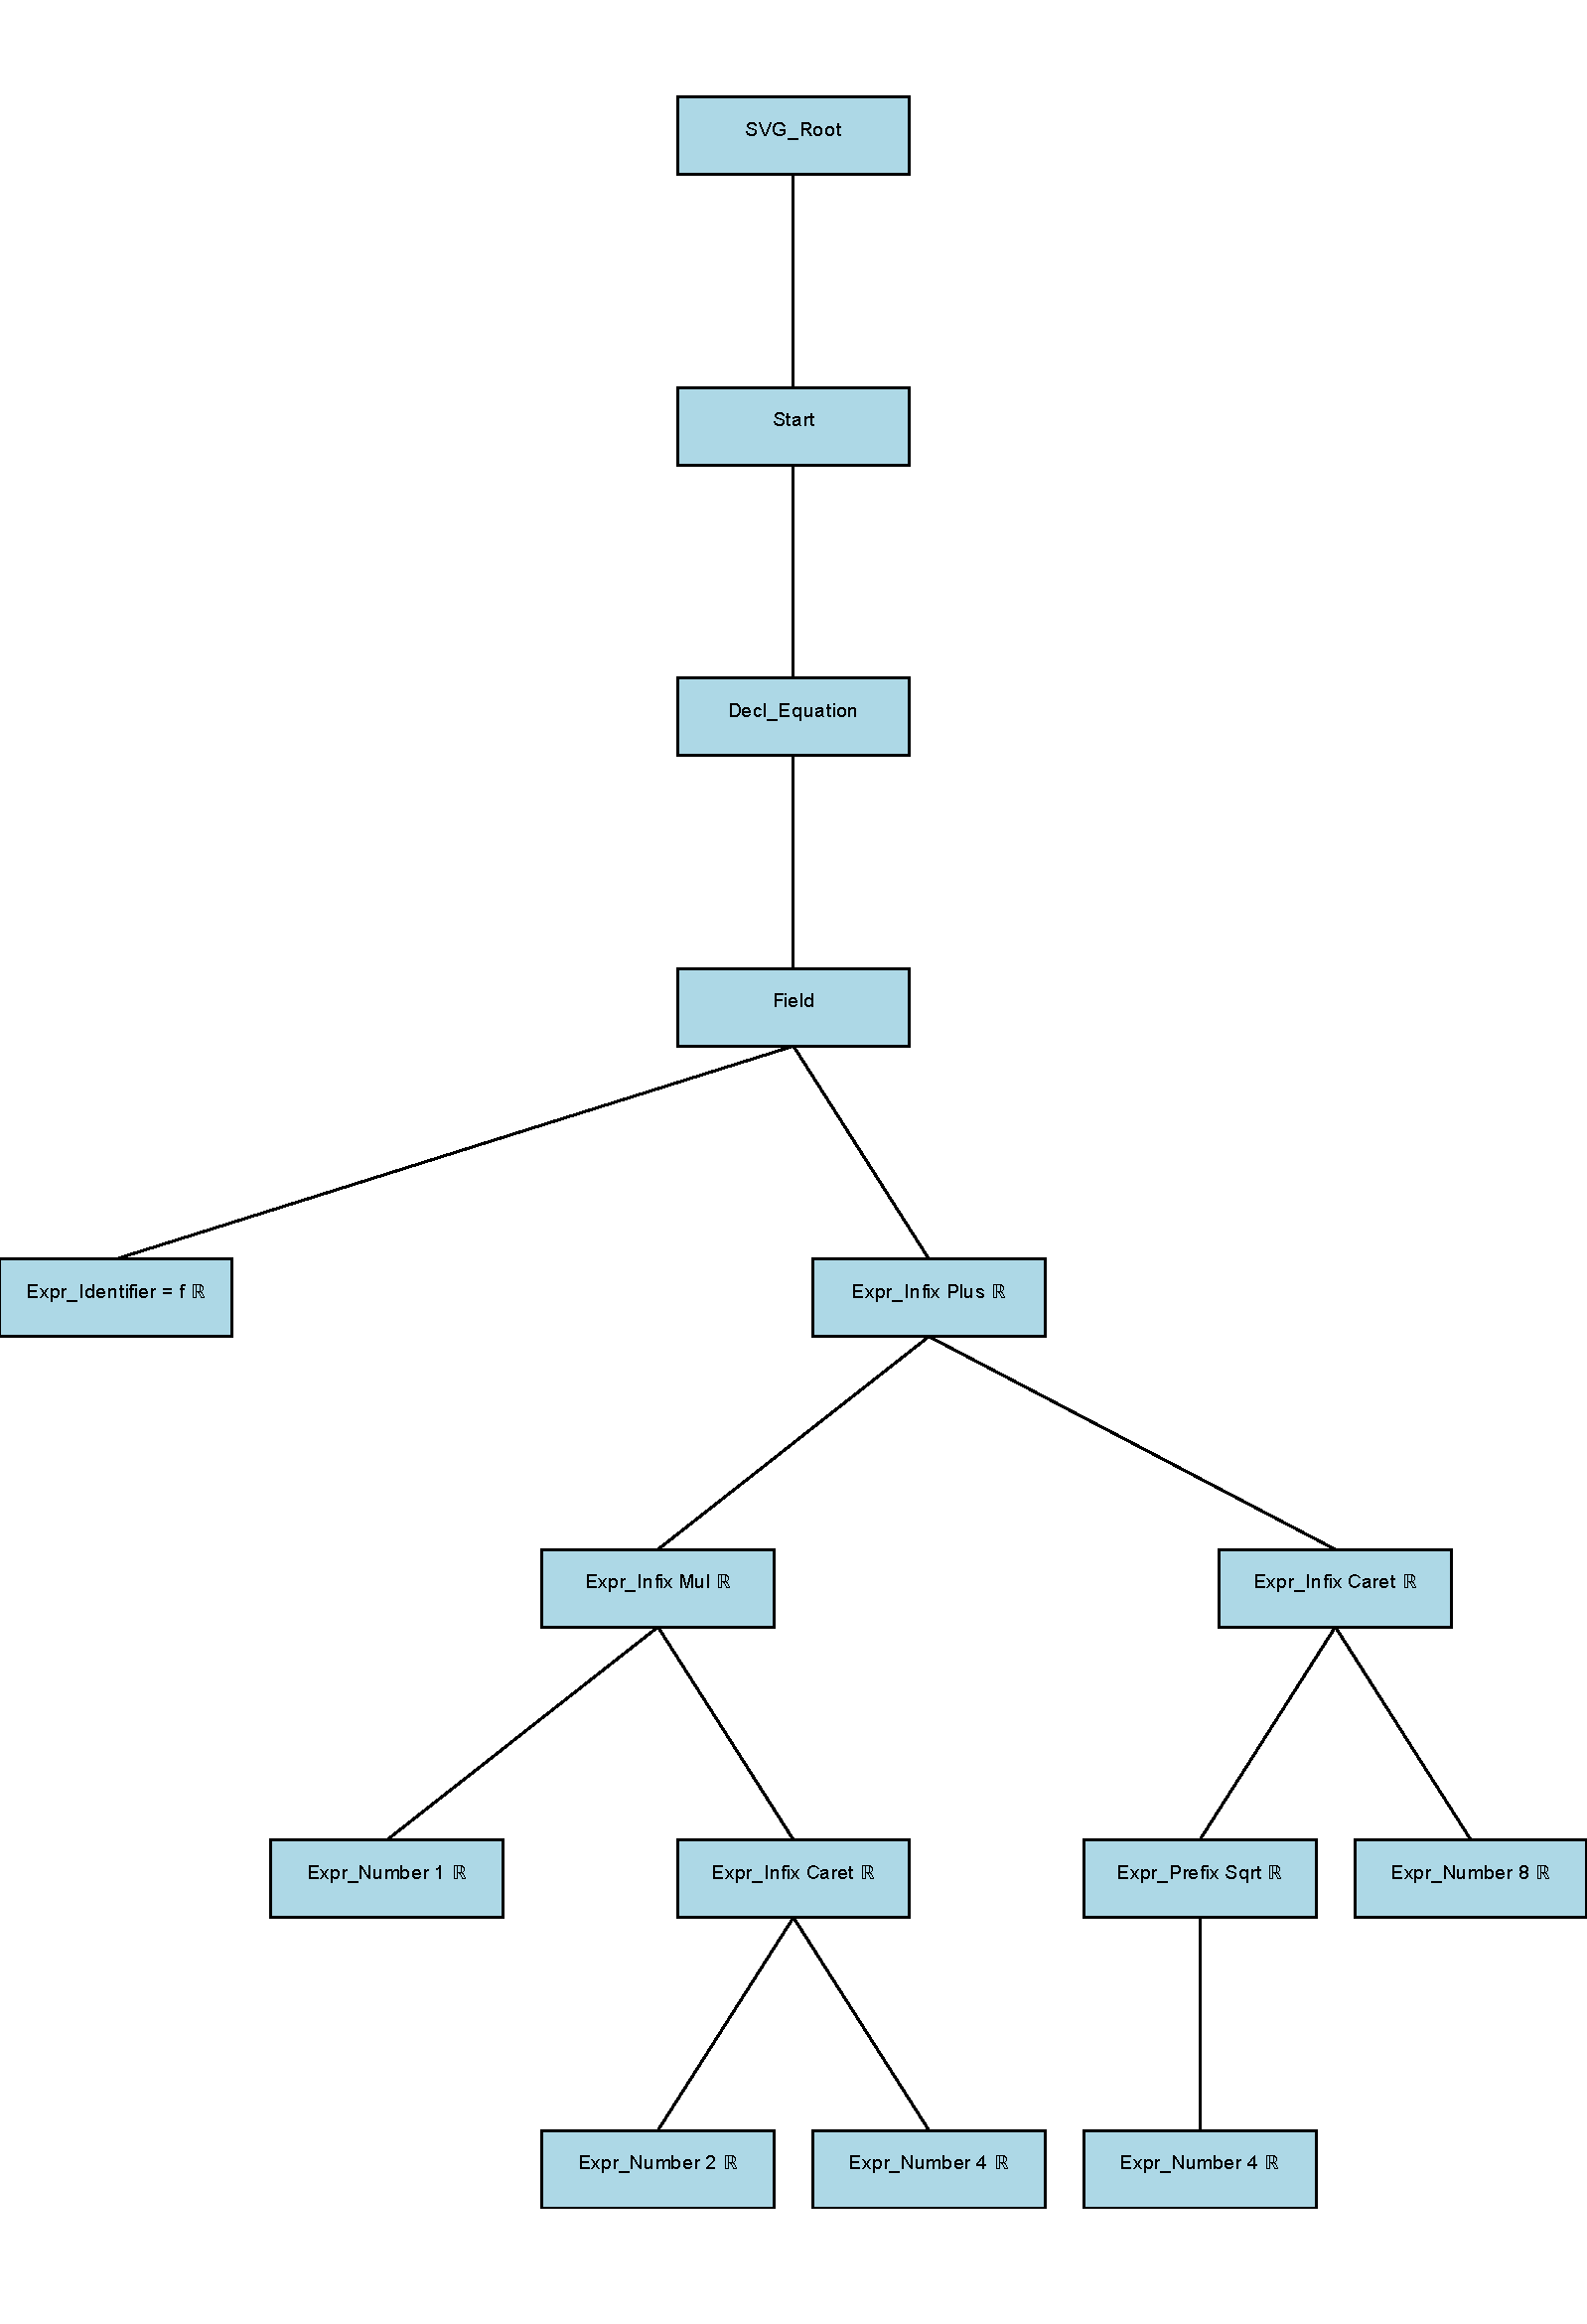
\includegraphics[scale=0.64]{./Imagens/svg.pdf}
    \end{center}
\end{figure}



% Temos dois tipos de validação dessa precendencia para garantir corretude de implementação de Pratt Parser, uma visual e outra automatica.
% Como mostrado em \autoref{tab-token-precedence} usamos uma tabela para definir a priopridade de operadores,
%
%
% ```
% \begin{equation}
% opertattions ungrouped
%
% \end{equation}
% ```
% Já se agruparmos certas operações, temos e o SVG gerado é diferente mostrando mostrando-se util em auxiliar o desenvolvimento.
%
%
% ```
% \begin{equation}
% grouped
% \end{equation}
% ```
% A maneira automatica é feita utilizando tested que gerandados sobre os casos, cada caso tem um entrada dada e saida esperada. A entrada é uma equação em string, a saída é uma string com a mesma, mas com a ordem de operação explicitamente citada através de parensentese. à Medida que o compialdor foi sendo desenvolvido mais teste foram adicionado para previnir quebra do código a medida que o projeto foi avançando. Alguns exemplos se encontram em @@@ e a informação gerada após aplicar o texto esta em @@@. Adicionamos o parentese através de um outro modulo chamado ``walker``, nele temos acesso à funções como ``children`` que dado um nó abstrato, ele resolve qual o tipo resolvido e cria um array de nós, como extrair os filho de nós heterogeneos precisa ser abstraido, cada estruttura tem campos diferetnes como filho. Outra facilidade que esse pacote desenvolvido é o padrão visitador @@ pegar o padrão visitador que tem função que utiliza generics.
%
%
% ```odin
% SVG_Node :: struct{
%     name: string,
%     children: [dynamic]^SVG_Node,
% };
% ```
% Como mostrado em @@@ usamos uma tabela para definir a priopridade de operadores
% Criamos um tabela que define e atráves de uma função, podemos acessar esses valores
% dado um token temos o reusltado
% Temos dois tipos de validação dessa precendencia para garantir correture de implementação de Pratt Parser, uma visual e outra automatica.
% Para validação visual, foi implementado um função que gera uma imagem no formato ``svg`` da arvore contendo informação circulos, representados nós da AST, jutamente com textos subinscritos informados metadados sobre os nós, como o tipo de operador, o tipo de nó, a string do indetificador  no caso de ser @etc
% Os nós próximo da raiz seriam implementados depois, já os proximos das folhas deve ser resolvikdos pprimeiros indicando um precedencia maior por exemplo
%
% Compilado para gerar a AST em SVG da equação @@, esperamos que '^' ocorra antes '*' que ocorra antes. Ao observar a arvore, notamos que o nó correspondente àoperação '^' ocorre.
%
% ```
% \begin{equation}
% opertattions ungrouped
%
% \end{equation}
% ```
% Já se agruparmos certas operações, temos e o SVG gerado é diferente mostrando mostrando-se util em auxiliar o desenvolvimento.
%
%
% ```
% \begin{equation}
% grouped
% \end{equation}
% ```
% A maneira automatica é feita utilizando tested que gerandados sobre os casos, cada caso tem um entrada dada e saida esperada. A entrada é uma equação em string, a saída é uma string com a mesma, mas com a ordem de operação explicitamente citada através de parensentese. à Medida que o compialdor foi sendo desenvolvido mais teste foram adicionado para previnir quebra do código a medida que o projeto foi avançando. Alguns exemplos se encontram em @@@ e a informação gerada após aplicar o texto esta em @@@. Adicionamos o parentese através de um outro modulo chamado ``walker``, nele temos acesso à funções como ``children`` que dado um nó abstrato, ele resolve qual o tipo resolvido e cria um array de nós, como extrair os filho de nós heterogeneos precisa ser abstraido, cada estruttura tem campos diferetnes como filho. Outra facilidade que esse pacote desenvolvido é o padrão visitador @@ pegar o padrão visitador que tem função que utiliza generics.
%
%
% ```odin
% SVG_Node :: struct{
%     name: string,
%     children: [dynamic]^SVG_Node,
% };
% ```
%
%
% \subsection{Testes}
%
%
% Foi desenvolvida uma série de testes que  abrangem vários aspectos da funcionalidade do \textit{parser}, incluindo geração de árvore de sintaxe, precedência de operadores e interpretação semântica.
%
%
% \subsubsection{Geração de Árvore de Sintaxe}
%
%
% Um aspecto crucial dos testes envolve verificar a correta geração de árvores sintáticas a partir de expressões de entrada. Os testes são projetados para cobrir diferentes cenários, incluindo operações aritméticas simples, expressões complexas com sub-expressões aninhadas e chamadas de funções. São eles:
%
%
% \begin{itemize}
%     \item O manuseio correto de operadores unários e binários, garantindo a precedência e associatividade adequadas.
%     \item A representação precisa de chamadas de função e seus argumentos dentro da árvore de sintaxe.
%     \item O agrupamento adequado de expressões dentro de parênteses para confirmar regras de precedência.
% \end{itemize}
